\documentclass[11pt, prl, reprint, aps, floatfix]{revtex4-1}

%Packages
\usepackage{amsmath}
\usepackage{mathrsfs}
\usepackage{graphicx}
\usepackage{float}
\usepackage{tikz}
\usepackage{standalone}
\usepackage{grffile}
\usepackage{cleveref}
\usepackage{todo}
\usepackage{physics}
\usepackage{tensor}
% \usepackage{todonotes}
\graphicspath{ {../../images/Thesis/} {../../images/Thesis/Background/} {../../images/Thesis/Background/qpFunctions/} {../../images/Thesis/carmichaelPaper/} {../../images/Thesis/bishopPaper/} }

%Operator,math and QM shorthands
\newcommand{\ham}{\hat{\mathscr{H}}}
\newcommand{\cre}{{\hat{a}^\dagger}}
\newcommand{\ann}{\hat{a}}
\newcommand{\atann}{\hat{\sigma}_-}
\newcommand{\atcre}{\hat{\sigma}_+}
\newcommand{\dens}{\hat{\rho}}
\newcommand{\bratens}[2]{\bra{#1} \otimes\bra{#2}}
\newcommand{\kettens}[2]{\ket{#1} \otimes\ket{#2}}
\newcommand{\qexp}[1]{\langle #1 \rangle}
\newcommand{\schro}[2]{i \hbar\ket{#1} = #2 \ket{#1}}
\newcommand{\Epsilon}{\mathcal{E}}
\newcommand{\gpr}{\iint_{\alpha, \beta \in \mathscr{D}}P \left( \alpha, \beta \right) \hat{\mathscr{J}} \dd{\mu}(\alpha, \beta)} 
\newcommand{\lindblad}[2]{\mathscr{L}_{#1}[#2]}
\newcommand{\hres}[1]{\hat{R}^\dagger(#1) \hat{S} +\hat{S}^\dagger \hat{R}(#1)}

%   General parameters, for ALL pages:
\renewcommand{\topfraction}{0.9}    % max fraction of floats at top
\renewcommand{\bottomfraction}{0.8}    % max fraction of floats at bottom
%   Parameters for TEXT pages (not float pages):
\setcounter{topnumber}{2}
\setcounter{bottomnumber}{2}
\setcounter{totalnumber}{4}     % 2 may work better
\setcounter{dbltopnumber}{2}    % for 2-column pages
\renewcommand{\dbltopfraction}{0.9}    % fit big float above 2-col. text
\renewcommand{\textfraction}{0.07}    % allow minimal text w. figs
%   Parameters for FLOAT pages (not text pages)

\begin{document}
\begin{abstract}
   This project is an investigation of the Jaynes-Cummings system in the presence of coherent drive and dissipation via various mechanisms, with particular focus on the parameter regimes of superconducting circuit QED.
We investigate the system in a variety of parameter regimes, and in the analysis is uncovered bistability in phase and amplitude, non-equilibrium phase transitions and non-classical states of light.
We investigate the conditions under which bimodality develops, and contrast the semiclassical regime, in which quantum fluctuation of the system is neglected, and the fully quantum regime, which we access using numerical simulations.
We also investigate analytical results for the quantum Kerr oscillator of \cite{Drummond1979} and \cite{Kheruntsyan1999}, and investigate the extent to which a perturbative expansion in the excitation number for the Jaynes Cummings oscillator admits these results as descriptions of our system. 

\end{abstract}
\title{Phase Transitions and Bimodality in the Dissipative-Driven Jaynes-Cummings Model}
\author{Fergus Barratt, Physics, UCL}
\affiliation{First Supervisor: Themis Mavrogordatos, Second Supervisor: Marzena Szymanska}
\date{\today}
\maketitle

\tableofcontents

\clearpage

\begin{figure}
  \includegraphics[width=\textwidth]{declaration.pdf}
\end{figure}

\clearpage

../tex/thesis/other/introduction.tex
%------------------------------------------------------------------------
%% Background.tex

\section{The Statistical Interpretation of Quantum Mechanics\cite{Breuer2002}}
Consider a statistical ensemble $\varepsilon$ consisting of a suitably large number N of identically prepared quantum systems
\begin{equation}
  \varepsilon = \left\{S^1, S^2, \ldots, S^N\right\}
\end{equation}
Such a statistical ensemble represents a particular set of experimental conditions, whose realisation in each instance generates a particular member $S^i$ of  $\varepsilon$

The first postulate of the statistical interpretation of quantum mechanics is that a complete characterisation of such a statistical ensemble can be represented by a normalised state vector $| \psi \rangle$ in an associated Hilbert space $\mathcal{H}$

The second postulate is that all the possible outcomes of measurements on such an ensemble are represented by self-adjoint operators on $\mathcal{H}$.
The outcome of the measurement corresponding to an operator $\hat{R}$ represents a real valued random variable R with cumulative distribution function $F_{\hat{R}}$ defined via the family of orthogonal projection operators that constitute the spectral decomposition of $\hat{R}$:
\begin{equation}
  \hat{R} = \int_{-\infty}^\infty r \dd{E_r}
\end{equation}
as
\begin{equation}
  F_{\hat{R}} = \expval{E_r}{\psi}
\end{equation}
This characterisation of the possible statistical variation of a quantum system is not yet complete, for it neglects classical uncertainty associated with which statistical ensemble $\varepsilon$ represents a given quantum system.
To generate the most general possible representation of a quantum statistical ensemble, a number of possible quantum ensembles $\varepsilon_\alpha$ of the above type are mixed with weights $w_\alpha$ (these weights are probabilities in the classical, not quantum sense).
A self-adjoint operator now yields a random variable R with cumulative distribution function
\begin{equation}
  F_{\hat{R}} = \sum_\alpha w_\alpha \expval{E_r}{\psi_\alpha} 
\end{equation}
for convenience, the \emph{density operator} $\dens$ can be introduced thus
\begin{equation}
  \dens = \sum_\alpha w_\alpha \ketbra{\psi_\alpha}{\psi_\alpha}
\end{equation}
and the cumulative distribution written:
\begin{equation}
  F_{\hat{R}} = \tr(E_r \dens)
\end{equation}
by a similar mixing argument and using the spectral decomposition of $\hat{R}$ the mean and variance of the random variable associated with $\hat{R}$ as above are as follows
\begin{align}
       \ev{\hat{R}} &= \tr(\hat{R} \dens ) \\
\text{var}(\hat{R}) &= \ev{\hat{R}^2} - {\ev{\hat{R}}}^2
\end{align}
The density matrix constitutes a complete description of the statistical properties of an open quantum system.
Thus, the dynamics of such a system can be described by the time evolution of its density operator.


../tex/thesis/background/sections/masterequation.tex

\section{Quasi-Probability Distributions}
Probability distributions in the classical theory of probability are subject to 3 important restrictions, which derive from the Kolmogorov axioms on the system probability measure.
The transition to a quantum theory of probability relaxes one or more of these axioms, and quasi-probability distributions result-these are not necessarily everywhere positive, and regions integrated under such distributions do not in general represent mutually exclusive states as do the analogous regions under true probability distributions.
This corresponds to the relaxation of the first and third of Kolmogorov's axioms.

Several different quasi-probability distribution representations are possible \cite{Walls2008}, and to each is associated a theorem known as the \emph{Optical equivalence theorem} \cite{Sudarshan1963}, for a power series of annihilation and creation operators in a given ordering.
The optical equivalence theorem is concisely stated as follows
\begin{equation}
	\langle g_{\Omega} (\alpha, \alpha^*) \rangle = \langle g_{\Omega} (\hat{a}, \cre) \rangle
\end{equation}
with $g_\Omega$ some power series of $\hat{a}$ and $\cre$, and $\Omega$ the ordering of that power series.
That is to say, the expectation of a power series of the operators $\hat{a}$ and $\cre$ is the same as the expectation value of the same power series with annihilation and creation operators replaced by complex eigenvalues $\alpha$ and $\alpha^*$ respectively, with regard to the appropriate quasiprobability distribution for that operator ordering.
The quasiprobability distributions for each ordering are listed below.

Quasi-probability distributions arise naturally when considering representations of the density operator.
The density operator is in general defined with regards to a complete orthonormal set of projection operators.
However, a diagonal representation of the density operator in terms of an \emph{overcomplete} set of non-orthogonal projectors is also always possible \cite{Sudarshan1963}, and the corresponding representation is in certain systems conceptually and computationally simpler.
The relevant overcomplete set in quantum optics is the set of coherent states of the electromagnetic field defined as the right eigenstates of the annihilation operator
\begin{equation}
\alpha | \alpha \rangle = \ann | \alpha \rangle
\end{equation}
\subsection{Normal Ordering}
An operator ordering is \emph{normal} if in all products of annihilation and creation operators, all creation operators come before annihilation operators \cite{Mandl2010} The Glauber-Sudarshan P function \cite{Cahill1969}:
\begin{equation}
	\dens = \int P(\alpha) | \alpha \rangle \langle \alpha | d^2 \alpha
	\end{equation}
        where $\dd[2]{\alpha} = \dd{Re\{\alpha \}}\dd{Im\{\alpha \}}$, is used for evaluating expectations of normally ordered power series:
\begin{equation}
  \langle \hat{a}^{\dagger n} \hat{a}^{m}  \rangle = \int \alpha^n \alpha^m P (\alpha, \alpha^*) \dd[2]{\alpha}
\end{equation}
P ($\alpha$) does not in general admit an interpretation as a classical probability distribution.
However, the transition between quantum and classical systems is most clearly visible in the P representation; any system with a classical analogue (a coherent state, a chaotic state) has a non-negative, classically interpretable P function, and any with no classical analogue (Fock states, or states exhibiting squeezing, antibunching) will have a P function which is either negative or more singular than delta function.
This statement is not generally true for other quasiprobability distributions \cite{Mandel1995}
\subsubsection{General procedure for evaluating P($\alpha$)}\label{mehta}
There exists a general expression for evaluating the P-function that yields a well-behaved function whenever such a function is possible.
 \cite{Mehta1967}:
\begin{equation}
	P(\alpha) = \frac{1}{\pi^2} \int d^2 \beta \bra{-\beta} \dens \ket{\beta} e^{|\beta|^2} e^{\beta^* \alpha -\alpha^* \beta}
\end{equation}
It is a necessary and suffient condition for this expression for P ($\alpha$) to be standard function that the function $ \bra{\beta} \dens \ket{\beta} e^{|\beta|^2} $ be square integrable.
Should it not be square integrable P ($\alpha$) can only be understood in the context of generalised function theory.
\subsection{Antinormal Ordering}
\emph{Antinormal} ordering is the inverse of normal ordering, in that annihilation operators appear before creation operators.
The associated quasi-probability distribution is the \emph{Husimi-Q Function} \cite{Husimi1940}, defined as the diagonal matrix elements of the density operator in a pure coherent state
\begin{equation}
	Q = \frac{\langle \alpha | \dens | \alpha \rangle}{\pi}
	\label{qdef}
\end{equation}
The Q function is a nonnegative, the density function being a positive operator.
It is also bounded above
\begin{equation}
	Q \leq \frac{1}{\pi}
\end{equation}
Antinormally ordered expectation values can be evaluated as follows:
\begin{equation}
  \langle \hat{a}^n \hat{a}^{\dagger m}  \rangle = \int \alpha^n \alpha^m Q (\alpha, \alpha^*) \dd[2]{\alpha}
\end{equation}
The Q function exists for states which admit no P representation, and unlike the P or W function is always positive.
It does not however always lead to a Fokker-Planck equation with a positive-definite diffusion matrix. 
\subsection{Symmetric Ordering}
The first quasi-probability distribution to be introduced and the most popular in the literature is the \emph{Wigner Function} \cite{Wigner1932} , which satisfies the OET for symmetrically ordered products: those of the form $\frac{\ann \cre + \cre \ann}{2}$
True probability distributions for generalised position and momentum are only possible independently $\rho(x) = |\braket{x}{\psi}|^2$, $\rho(p) = |\braket{p}{\psi}|^2$.
This is fundamental principle of quantum mechanics.
A joint statistical treatment is however available through the Wigner quasi-probability distribution
\begin{equation}
  W(X_1, X_2) = \frac{1}{4 \pi} \int_{-\infty}^\infty \dd{X} e^{\frac{-iXX_2}{2}} \bra{X_1+X} \dens \ket{X_1-X}
\end{equation}
Expressed in terms of the generalised position and momentum in quantum optics: the field quadratures defined $\alpha = X_1 + iX_2$.
Integrating over either quadrature yields the true probability distribution in the other quadrature.
The Wigner function is defined as the \emph{Wigner transform} of the density matrix, a general invertible transformation taking operators to functions on phase space.
Its inverse, the \emph{Weyl transform}, returns functions to operators.
The phase space formulation of quantum mechanics in its original form involves propagating such functions in time using Moyal's Evolution Equation \cite{Curtright2011}.
This same formalism is equivalently applied  through different integral transforms to the other representations.
\subsection{Characteristic Functions}
The above functions are equivalently derived from the antinormal, normal, and symmetric characteristic functions, defined as follows:
\begin{align}
	\chi_{A} (\eta) &= tr\{\dens e^{-\eta^* \hat{a}}e^{\eta \cre } \} \\
	\chi_{N} (\eta) &= tr\{\dens e^{\eta \cre}e^{-\eta^* \hat{a} } \} \\
	\chi_{S} (\eta) &= tr\{\dens e^{\eta^* \hat{a}-\eta \cre } \}
\end{align}
with the corresponding quasiprobability distributions retrieved as the inverse Fourier transform of the corresponding characteristic function
\begin{equation}
 	\{P|Q|W\} = \hat{\mathscr{F}}^{-1} [\chi_{\{N|A|S\}}]
\end{equation}
The existence of the inverse transform is necessary condition for the existence of a particular representation in terms of non-generalised functions.
\subsection{Coherent State Representations}
The form of the density matrix for a system in pure coherent state $ | \alpha_0 \rangle $  is:
\begin{equation}
 	\dens = | \alpha_0 \rangle \langle \alpha_0 |
\end{equation}
\subsubsection{P-function}
From the properties of the delta function, the form of the P-function is evident:
\begin{equation}
	P(\alpha) = \delta^2(\alpha-\alpha_0)
\end{equation}
\subsubsection{Q-function}
The Q-function is evaluated from the definition:
\begin{equation}
	Q(\alpha) = \frac{\langle \alpha | \alpha_0 \rangle \langle \alpha_0 | \alpha \rangle}{\pi} = \frac{{|\langle \alpha | \alpha_0 \rangle |}^2}{\pi} =  \frac{e^{-{|\alpha_0 - \alpha |}^2}}{\pi}
\end{equation}
\subsubsection{Wigner Function}
The Wigner function is recovered from the Wigner transform of $\ket{\alpha_0}\bra{\alpha_0} = \ket{X_1+iX_2}\bra{X_1+iX_2}$
\begin{equation}
	W(x_1, x_2) = \frac{2}{\pi} e^{-\frac{1}{2}[{(x_1-X_1)}^2+{(x_2-X_2)}^2]}
\end{equation}
\begin{figure}[!htb]
  \begin{minipage}{0.5\linewidth}
          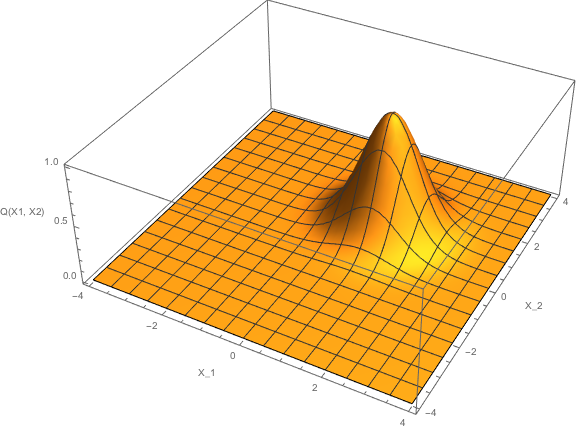
\includegraphics[width=\linewidth]{Q Function-Coherent.png}
	\end{minipage}%
  \begin{minipage}{0.5\linewidth}
          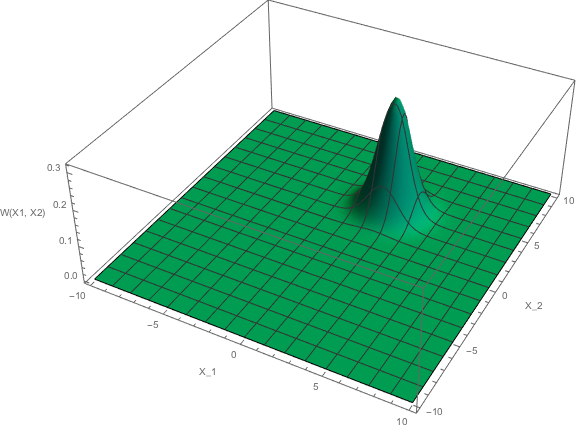
\includegraphics[width=\linewidth]{W Function-Coherent.png}
    \end{minipage}
  \caption{(a) Q function (orange) and Wigner Function (green) for the coherent states $\alpha = 1+i$ and $\alpha = 5+3i$}
\end{figure}
\subsection{Fock state representations}
\subsubsection{P-function}
Since Fock states have no classical analogue, we would expect the P function associated with the Fock state density matrix $\ket{n}\bra{n}$ should be highly singular or negative.
From \cite{Mehta1967}  P ($\alpha$) is non-singular (not more singular than a $\delta$-function) if and only if $ \bra{\beta} \dens \ket{\beta} e^{|\beta|^2} $ is square integrable.
But, using the Fock state expansion of the coherent states
\begin{align}
	 \bra{\beta} \dens \ket{\beta} e^{|\beta|^2}  &= e^{-|\beta|^2} \sum_{k=0}^\infty \frac {{\beta^*}^k}{k!} \braket{k}{n}\braket{n}{k} \sum_{k=0}^\infty \frac {\beta^k}{k!}e^{|\beta|^2} \\ &= e^{-|\beta|^2} \frac{|\beta|^{2n}}{{n!}^2} e^{|\beta|^2} \\ &= \frac{|\beta|^{2n}}{{n!}^2}
\end{align}
Which is square integrable for no value of n.

A representation in terms of a class of generalised functions called \emph{tempered distributions} is possible\footnote{Specifically, in terms of the derivatives of a Dirac delta function \cite{Gerry2005}}, but the behaviour of such objects makes them difficult to work with.
\subsubsection{Q-function}
Despite the pathological Fock state P-function the Q-function follows simply from the definition
\begin{align}
	 Q(\alpha) = \bra{\alpha} \dens \ket{\alpha}  &= \sum_{k=0}^\infty \frac {{\alpha^*}^k}{k!} \braket{k}{n}\braket{n}{k} \sum_{k=0}^\infty \frac {\alpha^k}{k!}e^{-|\alpha|^2} \\ &= \frac{|\alpha|^{2n}}{{n!}^2} e^{-|\alpha|^2}
\end{align}
\begin{figure}[!htb]
	\begin{minipage}[b]{.5\linewidth}
        \centering \large 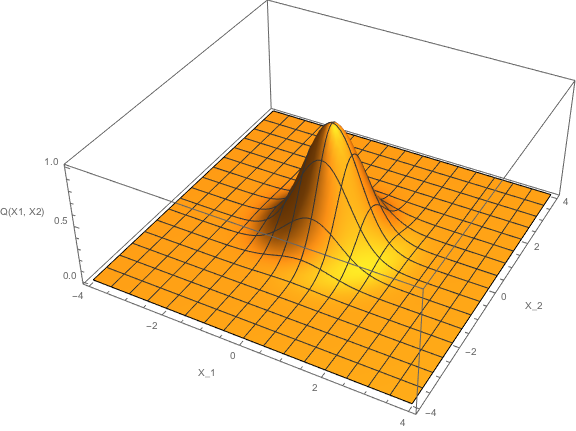
\includegraphics[width=1\linewidth]{Q Function-n=0.png}
	\end{minipage}%
	\begin{minipage}[b]{.5\linewidth}
		\centering\large 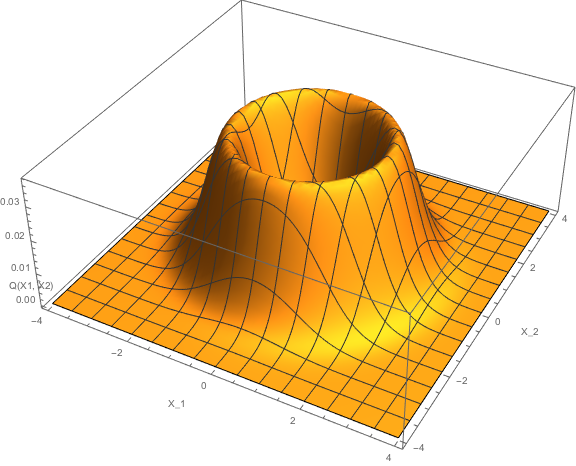
\includegraphics[width = 1\linewidth]{Q Function-n=3.png}
	\end{minipage}
  \caption{Fock State Q Functions for n=0 and n=5}\label{Qfunctions}
\end{figure}
\subsubsection{Wigner function}
The Wigner transform of $\ket{n}\bra{n}$ is \cite[65]{Walls2008}
\begin{equation}
	W(x_1, x_2) = \frac{2}{\pi} {(-1)}^n \mathscr{L}_n(4(x_1^2+x_2^2))e^{-2(x_1^2+x_2^2)}
\end{equation}
Where $\mathscr{L}_n$ is the nth Laguerre Polynomial.
\begin{figure}[!htb]
	\begin{minipage}[b]{.5\linewidth}
		\centering \large 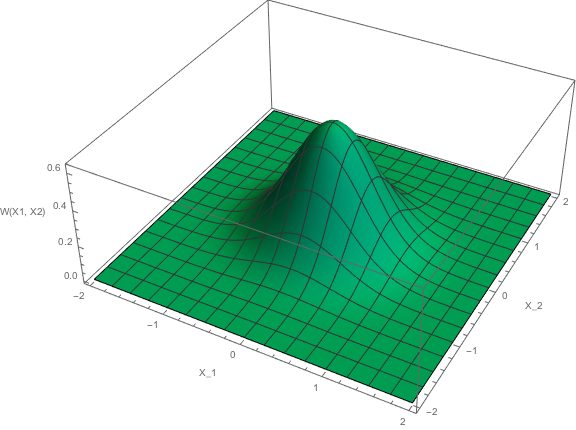
\includegraphics[width=1\linewidth]{W Function-n=0.png}
	\end{minipage}%
	\begin{minipage}[b]{.5\linewidth}
		\centering\large 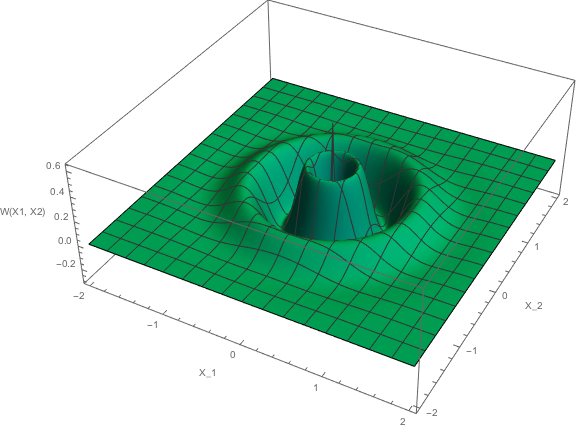
\includegraphics[width = 1\linewidth]{W Function-n=10.png}
	\end{minipage}
	\caption{Fock State Wigner Functions for n=0 and n=10}\label{Wfunctions}
\end{figure}
\subsection{Generalised P Representations}
\label{gen_p}
Any density operator admits a diagonal P representation in terms of distributions, which are computationally and conceptually complicated.
The overcompleteness of the coherent states does not sufficiently restrict the P function, and thus they are not unique.
For this purpose the R representation was proposed \cite{Glauber1963a}. 
This representation does not generally yield positive definite Fokker-Planck diffusion matrices \cite{Walls2008}, and as such it has not seen much use.\\

Introducing an additional complex variable for a coherent basis {$\ket{\beta}_{\beta\in\mathbb{C}}$}, a measure $d\mu(\alpha, \beta)$ and an integration domain $\mathscr{D}\subset\mathbb{C}\times\mathbb{C}$ defines a family of representations of the density matrix, which have had substantial analytical success
 \cite{Drummond1979}.
This formalism is due to \cite{Drummond1980}.
The extension goes 
\begin{equation}
  \dens = \iint_{\alpha, \beta \in \mathscr{D}}P \left( \alpha, \beta \right) \hat{\mathscr{J}} 
  \dd{\mu \left( \alpha, \beta \right)}
          \label{gen_p_rep}
\end{equation}
with
\begin{equation}
  \hat{\mathscr{J}} = \frac{\ket{\alpha}\bra{\beta^*}}{\braket{\beta^*}{\alpha}} 
\end{equation}
We trade a real (quasi-)probability function over a real (classical) phase space, for a (generally) complex function of two complex variables, on a complex phase space.
\subsubsection{Diagonal} 
The measure that recovers the diagonal P representation is
\begin{equation}
  d\mu(\alpha, \beta) = \delta(\alpha-\beta^*)d^2 \alpha d^2 \beta
\end{equation}
$\alpha$ and $\beta = \alpha^*$ now take values on a two-dimensional subset of the complex plane ($\mathbb{C}\times\mathbb{C}$) - the familiar real phase plane.
\subsubsection{Complex}
Letting $\beta, \alpha$ vary independently on two different complex contours $\mathscr{C}, \mathscr{C}'$, and taking as measure
\begin{equation}
  d\mu\left(\alpha, \beta\right) = \dd{\alpha} \dd{\beta}
\end{equation}
The corresponding P function can take complex values.
This representation has been used to derive the photon number distribution of a cavity containing a nonlinear medium \cite{Drummond1979}.
\subsubsection{Positive}
We consider a surface integral over the whole $\alpha$-$\beta$ plane
\begin{equation}
  d \mu(\alpha, \beta) = \dd[2]{\alpha} \dd[2]{\beta}
\end{equation}
In this case the distribution is always positive, and always admits an interpretation as a genuine probability. 
\subsection{Stochastic Processes \& Fokker-Planck Equations}
\begin{equation}
  \pdv{t}P(\alpha, \beta) = (\partial_\mu A_\mu (\alpha, \beta) + \frac{1}{2} \partial_\mu \partial_\nu D_{\mu\nu}) P(\alpha, \beta) 
  \label{fokker_planck}
\end{equation}
Here we talk about stochastic processes and Fokker-Planck equations in quantum optics 
 \cite{Carmichael1992} 
 \cite{Carmichael2008} 
 \cite{Breuer2002} 
\subsection{Application}
The canonical quantisation of a system consisting of a nonlinear medium inside a cavity leads to a Hamiltonian of the form 
\begin{equation}
  \mathscr{H} = \hbar \delta_{cd} \cre \ann + \hbar \chi \cre{}^ 2 \ann{}^ 2 + \hbar \left( \ann \xi(t) + \cre \xi(t)^* \right) 
\end{equation}
after moving to a rotating frame at the drive frequency.
with $\chi$ a function of the third order anharmonicity of the medium and the electric field mode functions, $\delta_{cd}$ the detuning of the drive from the resonant frequency of the cavity, and $\xi(t)$ the time varying drive envelope \cite{Drummond1979}.
We form a master equation with lindblad dissipators $\mathscr{L}_{\kappa}[\dens]$ and $\mathscr{L}_{\text{therm}}[\dens] = \mathscr{L}_{\bar{n}+1}[\dens] +  \mathscr{L}_{\bar{n}}[\dens]$ representing the dissipation of the cavity field through the mirrors, and interaction with a finite temperature environment with mean photon number $\bar{n}$ respectively.
\begin{equation}
  \dot{\dens} = i\hbar\comm{\ham}{\dens} + \mathscr{L}_{\kappa}[\dens] + \mathscr{L}_{\text{therm}}[\dens]
\end{equation}
We insert the generalised P representation, defined in \cref{gen_p_rep}.
\begin{align}
  \pdv{t} P(\alpha, \beta)  &= \Bigg(\pdv{\alpha} (\kappa \alpha + 2 \chi^* \alpha^2 \beta - \xi(t) )\\ 
                            &- \chi(t) \pdv[2]{\alpha} \alpha^2\\
                            &+ \pdv{\beta} (\kappa^* \beta + 2\chi^* \beta^2 \alpha - \xi^*(t))\\
                            &- \chi^*(t) \pdv[2]{\beta} \beta^2\\
                            &+ (2(\kappa - i\delta_{cd})\bar{n} + \Gamma_E ) \pdv{}{\alpha}{\beta}\Bigg) P(\alpha, \beta)
\end{align}
where we have introduced a term $\Gamma_E$ which accounts for the fluctuation of the drive.

\cite{Haken1975} provides a condition under which exact steady state solutions may be attained. It follows:
For a Fokker-Planck equation of the standard form \cref{fokker_planck}, the potential
\begin{equation}
  V_\rho(\alpha, \beta) = D_{\rho\nu}(\alpha, \beta)^{-1} (2A_\nu(\alpha, \beta) + D_\sigma D_{\nu\sigma}(\alpha, \beta))
\end{equation}
must satisfy
\begin{equation}
  \partial_\mu V_\nu = \partial_\nu V_\mu
\end{equation}
In our case one can verify that the condition is satisfied in the limit $\Gamma = 2(\kappa - i\delta{cd})\bar{n} + \Gamma_E \ll \abs{\chi( \bar{n} + \bar{n}_{\text{cav}} )}$, where $\bar{n}_{\text{cav}}$ is the average photon number in the cavity.

In this limit we can neglect $\Gamma$, the off-diagonal elements of the diffusion matrix for the fokker-planck equation.
The diffusion matrix thus becomes positive-definite, and we have for the drift A and diffusion D
\begin{align}
  A  &= \begin{pmatrix}
  \mqty{(\kappa - i\delta_{cd})\alpha + 2\chi\alpha^2 \beta - \xi(0)\\ (\kappa - i\delta_{cd})\alpha + 2\chi^* \beta^2 \alpha - \xi^*(0)}
       \end{pmatrix}\\
  D  &= \begin{pmatrix}
       \mqty{-2\chi\alpha^2 & 0 \\ 0 & -2 \chi^* \beta^2 }
       \end{pmatrix}
\end{align}
from which the potential condition can be easily verified. 
From here, \cite{Haken1975} gives a prescription for evaluating the P function from the potential
\begin{equation}
  P(\alpha, \beta) = \exp \left( - \int^\alpha \int^\beta \dd{\beta}\dd{\alpha} V_\mu (\alpha, \beta) \right)
\end{equation}
for our parameters, the solution is 
\begin{equation}
  P(\alpha, \beta) = \alpha^{\frac{\kappa-i\delta_{cd}}{\chi}-2} \beta^{{\left[\frac{\kappa-i\delta_{cd}}{\chi}\right]}^*-2}\exp{\frac{\xi(0)}{\chi}\left(\frac{1}{\alpha} + \frac{1}{\beta}\right) + 2\alpha\beta}
\end{equation}
\subsubsection{Moments}
The generalised P function has normal ordered expectation values as its moments, just as the diagonal representation.
On the diagonal integration domain (i.e. $\ket{\alpha} \text{for } \alpha \in \mathbb{C}$) with the diagonal measure setting $\beta = \alpha^*$, there is a term in $\exp{\alpha\beta} = \exp{\abs{\alpha}^2}$ for which the integral on the domain is divergent.
We take instead the complex measure, on two different contours.
The moments of the distribution are the same as the normalisation integral but for the $\alpha$ and $\beta$ exponents.
We take a function with general exponents $c = (\kappa-i\delta_{cd}) / \chi + k $, $d = ((\kappa-i\delta_{cd}) /\chi)^*+q$, where $k, q \in \mathbb{N}$, and make the variable change $\gamma = \flatfrac{1}{\alpha}, \varphi = \flatfrac{1}{\beta}$
\begin{align*}
  P(\gamma, \varphi) &= \gamma^{-c-2} \varphi^{-d-2} \exp{\frac{1}{\gamma\varphi}} \exp{\frac{\xi(0)}{\chi}\left(\gamma + \varphi \right)}\\
                     &= \sum_{n=0}^\infty\flatfrac{\left(\frac{1}{\gamma\varphi}\right)^n}{n!} \times \gamma^{-c-2}\varphi^{-d-2} \exp{\frac{\xi(0)}{\chi}(\gamma+\varphi)}\\
                     &= \sum_{n=0}^\infty\flatfrac{2^n \gamma^{-c-2-n}\varphi^{-d-2-n} \exp{\frac{\xi(0)}{\chi}(\gamma+ \varphi)}}{n!}
\end{align*}
Integrating on contours $\mathscr{C}, \mathscr{C'}$
\begin{align*}
  I(c, d) = \iint_{\mathscr{C}, \mathscr{C}'} \dd{\gamma}\dd{\varphi} P(\gamma, \varphi) &= \sum_{n=0}^\infty\frac{1}{n!} \int_\mathscr{C} \dd{\gamma} \gamma^{-c-n} \exp{\frac{\xi(0)}{\chi}\gamma} \\ 
                                                                                 & \qquad \ \ \times \int_{\mathscr{C}'}\dd{\varphi} \varphi^{-d-n} \exp{\frac{\xi(0)}{\chi}\varphi}
\end{align*}
We take for the contours Hankel paths from $-\infty$ to $-\infty$, anticlockwise, enclosing the origin \cite{Drummond1979}. 
We have then gamma functions as in \cite{TISP}.
\begin{equation}
     \frac{1}{\Gamma(x)} = \left(\frac{t^{1-x}}{2\pi i}\right) \int_{\mathscr{C}} \dd{\eta}\eta^{-x} \exp{\eta x}
\end{equation}
thus
\begin{equation}
  I(c, d) = -4\pi^2 \sum_{n=0}^\infty \frac{2^n \{\flatfrac{\xi(0)}{\chi}\}^{c+d+2(n-1)}}{\Gamma(c+n)\Gamma(d+n)n!}
\end{equation}
using the form of the $_0F_2$ generalized hypergeometric function \cite{Slater1966} \cite{TISP}
\begin{equation}
  _0F_2(c, d, z) = \sum_{n=0}^\infty \left( \frac{ z^n \Gamma(c) \Gamma(d)}{\Gamma(c+n)\Gamma(d+n)n!} \right)
\end{equation}
we have 
\begin{equation}
  I(c, d) = \left( \frac{4\pi^2 \abs{\frac{\xi(0)}{\chi}}^{c+d-2}}{\Gamma(c)\Gamma(d)} \right) {}_0F_2 \left(c, d, 2\abs{\frac{\xi(0)}{\chi}}^2\right)
\end{equation}
Which gives expressions for all normally ordered moments 
\begin{equation}
  \ev{\cre{}^n \ann^m} = \displaystyle \frac{\displaystyle I\left(\frac{\kappa-i\delta_{cd}}{\chi}+n, \frac{\kappa+i\delta_{cd}}{\chi}+m\right)}{\displaystyle I\left(\frac{\kappa-i\delta_{cd}}{\chi}, \frac{\kappa+i\delta_{cd}}{\chi}\right)}
\end{equation}
particularly:
\begin{widetext}
  \begin{align}
    &\text{The cavity field: }\nonumber\\ 
    &\ev{\ann} = \frac{\chi}{\kappa-i\delta_{cd}} \abs{\frac{\xi(0)}{\chi}} {}_0F_2\left(1+ \frac{\kappa-i\delta_{cd}}{\chi}, \frac{\kappa+i\delta_{cd}}{\chi}, 2\abs{\frac{\xi(0)}{\chi}}^2\right) \Bigg/ {}_0F_2 \left(\frac{\kappa-i\delta_{cd}}{\chi}, \frac{\kappa+i\delta_{cd}}{\chi}, 2\abs{\frac{\xi(0)}{\chi}}^2\right)\label{field_duff}\\
    &\text{The 2nd order correlation function: }\nonumber\\
    g^{(2)}(0) =& \frac{\ev{\cre{}^2 \ann{}^2}}{\ev{\cre\ann}^2} =  \cfrac{(\kappa^2 + \delta_{cd}^2){}_0F_2 \left( \frac{\kappa - i \delta_{cd}}{\chi}, \frac{\kappa+i\delta_{cd}}{\chi}, 2\abs{\frac{\xi(0)}{\chi}}^2 \right) {}_0F_2 \left( \frac{\kappa-i\delta_{cd}}{\chi}+2, \frac{\kappa+i\delta_{cd}}{\chi}+2, 2\abs{\frac{\xi(0)}{\chi}}^2 \right)}{(\kappa^2 + \delta_{cd}^2 + 2 \kappa + 1) \left[{}_0F_2\left(\frac{\kappa-i\delta_{cd}}{\chi}+1, \frac{\kappa+i\delta_{cd}}{\chi}+1, 2\abs{\frac{\xi(0)}{\chi}}^2 \right)\right]^2} \label{g2_duff}
  \end{align}
\end{widetext}


../tex/thesis/background/sections/cqed.tex

\section{The Jayes-Cumming Hamiltonian}
In the Jaynes-Cummings model, a single cavity mode interacts with a two level system. 

We start with the total Hamiltonian
\begin{equation}
	\mathscr{H} = \mathscr{H}_A + \mathscr{H}_F +\mathscr{V}_{int}
\end{equation}
\subsection{The Dipole Approximation}
In full generality, the field will interact with all the higher order dipole moments of the atom.
However, given that the spatial variation of typical optical fields is minimal on the order of an atom ($\sim$ \AA), the interaction hamiltonian can be approximated by the interaction of the electric field only with the electric dipole moment of the atom
\begin{equation}
	\hat{\mathscr{V}}_{int} = -\vec{\hat{d}} \cdot \vec{\hat{E}}
\end{equation}
The quantized electromagnetic multimode vector potential in a medium can be expressed in the following way \cite[271--273]{Novotny2006}(we consider only a countable number of field modes, since we will put the field in a cavity)
\begin{equation}
	\hat{A} = \sum_{\vec{k}, \mu} \sqrt{\frac{\hbar}{2\omega_{\vec{k}} V \varepsilon_0}} (\vec{u}_{\vec{k}} \ann + \vec{u}^*_{\vec{k}} \cre )
\end{equation}
with $\vec{u}_{\vec{k}}$ orthogonal normal modes satisfying the wave equation:
\begin{equation}
	\nabla \times \nabla \times \vec{u}_{\vec{k}} = \frac{\omega_{\vec{k}}^2}{c^2}  \vec{u}_{\vec{k}}
\end{equation}
We consider only coupling to a single mode of the cavity field:
\begin{equation}
	\hat{A} =  \sqrt{\frac{\hbar}{2\omega_{\vec{k}} V \varepsilon_0}} (\vec{u}_{\vec{k}} \ann + \vec{u}^*_{\vec{k}} \cre )
\end{equation}
from which $\vec{E}$ for the mode is easily derived since (in the radiation gauge)
\begin{equation}
	\vec{\hat{E}} = -\frac{\partial}{\partial t}\vec{\hat{A}}
\end{equation}
\subsection{Two Level Approximation}
$\vec{\hat{d}} = e \vec{\hat{r}}$ can be expanded in the space of atomic levels by resolving unity on each side
\begin{equation}
	\vec{\hat{d}} = e \sum_{a, b} | a \rangle \langle a | \vec{\hat{r} }| b \rangle \langle b |
\end{equation}
since we consider only two levels, the sum can be truncated:
\begin{equation}
	\vec{\hat{d}} = e\{| 1 \rangle \langle 1|\vec{\hat{r}} | 1 \rangle \langle 1 | + | 1 \rangle \langle 1|\vec{\hat{r}} | 2 \rangle \langle 2 | + | 2 \rangle \langle 2|\vec{\hat{r}} | 1 \rangle \langle 1 | + | 2 \rangle \langle 2|\vec{\hat{r}} | 2 \rangle \langle 2 | \}
\end{equation}
we assume the atom has no permanent dipole moment and neglect terms of the form $| 1 \rangle \langle 1|\vec{\hat{r}} | 1 \rangle \langle 1 |$.
Expressing in terms of the atomic creation and annihilation operators
\begin{equation}
	\vec{\hat{d}} = (m\sigma_+ + m^* \sigma_-)
\end{equation}
where $m, m^*$ are the electric dipole matrix elements
\subsection{The Rotating Wave Approximation}
The free field hamiltonian, neglecting the zero point energy has the form
\begin{equation}
	\ham_F =  \hbar \omega \cre \ann
\end{equation}
The atom energy, neglecting centre of mass motion and considering only population inversion, in terms of the Pauli z matrix:
\begin{equation}
	\ham = \frac {1} {2} \hbar \omega_q \sigma_z
\end{equation}
where $\omega_q$ is the frequency of the bare atomic transition
Assuming sinusoidal mode functions with polarisation $\varepsilon_\Omega$, and incorporating constants into new dipole matrix elements $g = \frac{m \varepsilon_\Omega sin(Kz)} {2 \hbar}$, the total hamiltonian takes the form
\begin{equation}
	\ham = \hbar \omega \cre \hat{a} +\frac{1}{2} \hbar \omega_q \sigma_Z + \hbar (\ann +\cre)(g\atann+g^*\atcre)
\end{equation}
expanding the interaction term
\begin{align}
  \hat{\mathscr{V}}_{int} &= \hbar (\ann +\cre)(g\atann+g^*\atcre) \\
                          &=  \hbar (g \ann \atann + g^* \ann \atcre + g \cre \atcre +g^* \cre\atann)
\end{align}
moving to an interaction picture rotating at the transition frequency $\omega_q$ it can be seen that terms of the form $\atann \cre $ counterrotate with frequency $\omega + \omega_L$ and terms of the form $ \atann \ann$ co rotate with frequency given by the detuning $\omega-\omega_L$.
The rotating wave approximation is the assumption that the counterrotating terms will quickly average to zero on the system timescale, and thus can be dropped in the expansion of the interaction hamiltonian.
This approximation has broad application, especially at optical frequencies \cite, but it has its limits \cite{Dolce2006} \cite{Milonni1995} \cite{Biswas1990}.
\subsection{The Jaynes-Cumming Hamiltonian}
Applying all of the above leads to a hamiltonian $\ham_{JC}$ of the form:
\begin{equation}
	\ham_{JC} = \hbar \omega \cre \hat{a} +\frac{1}{2} \hat{\sigma}_Z \omega_q + \hbar g (\cre \atann + \hat{a} \atcre)
\end{equation}
\subsection{Solving the Jaynes Cumming system in the absence of drive}
\subsubsection{Bare states}
We first move to an interaction picture rotating with the bare system, partitioning the Hamiltonian
\begin{align}
	\ham_I &= \hbar \omega \hat{N}_e + \hbar(\frac{\omega_q}{2}-\omega)\hat{P}_E \\
	\ham_{II} &= -\hbar \Delta + \hbar g (\cre \atann + \hat{a} \atcre) \\
	\ham_{JC} &= \ham_I+\ham_{II}
\end{align}
with $\Delta = \omega-\omega_q$,   $\hat{N}_e = \ket{2} \bra{2} + \ket{1} \bra{2} $ the (conserved) electron number and $\hat{P}_E = \cre\ann + \ket{2}\bra{2} $ the (conserved) excitation number.

We consider evolution of the Jaynes-Cumming system in the absence of decay, dephasing and detuning, in the bare state basis.
Since the field only couples successive levels of the combined atom-field system, the state of the closed system can be described in the restricted two level Hilbert space
\begin{equation}
	\ket{\psi(t)} = C_1(t) \kettens{1}{g} + C_2(t) \kettens{0}{e}
\end{equation}
where $\ket{\psi}$ is understood to be an element of the atom-field Hilbert space.
We solve the interaction schrodinger equation to determine the time dependent coefficients $C_1(t)$ and $C_2(t)$
\begin{equation}
	\schro{\psi(t)}{\ham_{II}}
\end{equation}
and get two coupled differential equations for the level amplitudes:
\begin{align}
	\frac{d C_2(t)}{dt} &= -i g \sqrt{n+1}C_1(t)\\
	\frac{d C_1(t)}{dt} &= -i g \sqrt{n+1}C_2(t)
\end{align}
which are solved by
\begin{align}
  C_1(t) &= \cos(g\sqrt{n+1}t)\\
  C_2(t) &= \sin(g\sqrt{n+1}t)
\end{align}
\subsubsection{Dressed States}
The uninteracting hamiltonian 
\begin{equation}
  \mathscr{H}_{\text{bare}} = \hbar \omega_c + \hbar \omega_q \flatfrac{\sigma_z}{2}
\end{equation}
satisfies 
\begin{align}
  \mathscr{H} \ket{0, n} &= \hbar \left\{\frac{1}{2} \omega_q + \omega_c \right\} \ket{0, n}\\
  \mathscr{H} \ket{1, n} &= \hbar \left\{-\frac{1}{2} \omega_q + \omega_c \right\} \ket{1, n}
\end{align}
where $\ket{q, n} = \kettens{q}{n}$, $\{\ket{n}\}$ field fock states. 
The interacting hamiltonian
\begin{align}
  \mathscr{H}_I = \hbar g \left(\ann \atcre + \atann \cre\right)
\end{align}
couples only within pairs $\{\ket{0, n+1},\ \ket{1, n}\}$
We can consider the hamiltonian as acting only in the two dimensional space spanned by these states. 
In the matrix representation we have \cite{Meystre2007}
\begin{align*}
  \mathscr{H} &= \mathscr{H}_{\text{bare}} + \mathscr{H}_I \\
              &= \hbar \left(n+\frac{1}{2}\right) \omega_c 
  \begin{pmatrix}
    \mqty{1 & 0 \\ 0 & 1}
  \end{pmatrix}
              + \hbar / 2
  \begin{pmatrix}
    \mqty{\delta_{cq} & 2g\sqrt{n+1} \\ 2g\sqrt{n+1} & -\delta_{cq}}
  \end{pmatrix}
\end{align*}
The first matrix is obviously diagonal. 
The second is easily diagonalisable, with eigenvalues
\begin{align}
  \mathcal{E}_{-, n} &= \mathcal{E}_{\text{bare}} - \frac{1}{2} \hbar \sqrt{\delta_{cq}^2 + 4g^2 \left(n+1\right)}\\
  \mathcal{E}_{+, n} &= \mathcal{E}_{\text{bare}} + \frac{1}{2} \hbar \sqrt{\delta_{cq}^2 + 4g^2 \left(n+1 \right)}
\end{align}
where
\begin{equation}
  \mathcal{E}_{\text{bare}} = \hbar\left(n + \frac{1}{2}\right) \omega_c
\end{equation}
and eigenvectors
\begin{align}
  \ket{+}_n &= \cos(\theta) \ket{0, n+1} - \sin(\theta) \ket{1, n} \\
  \ket{-}_n &= \sin(\theta) \ket{0, n+1} + \cos(\theta) \ket{1, n} 
\end{align}
where
\begin{equation}
  \tan{2\theta} = -\frac{2g\sqrt{n+1}}{\delta_{qd}}
\end{equation}
These eigenstates are known as the \emph{dressed states}.
The atomic states are \emph{dressed} by the cavity field, and the energy levels are split by an amount $\hbar \sqrt{\delta_{cq}^2 + 4g^2\left(n+1\right)}$.
This is known as \emph{anti} or \emph{avoided} crossing.
We have the following relation between the dressed and bare level amplitudes
\begin{equation}
  \begin{pmatrix}
    \mqty{C_+(t) \\ C_-(t)}
  \end{pmatrix}
  =
  \mathcal{T}
  \begin{pmatrix}
    \mqty{C_{1, n} \\ C_{0, n+1}}
  \end{pmatrix}
\end{equation}
where
\begin{equation}
  \mathcal{T} = 
  \begin{pmatrix}
    \mqty{\cos(\theta) & -\sin(\theta) \\ \sin(\theta) & \cos(\theta) }
  \end{pmatrix}
\end{equation}
is a the unitary rotation matrix from one basis to the other.
From the time evolution operator representation of the schrodinger equation, after resolving unity with the dressed states we have for the bare state probability amplitudes. 
\begin{align*}
  \ket{\psi(t)} &= \exp{-i\mathscr{H}t/\hbar} \ket{\psi(0)}\\
                &= \sum_{n=0}^\infty \sum_{\pm} \exp{-i\mathscr{E}_{\pm, n}t/\hbar} \ket{\pm}_{n \ n}\bra{\pm}\ket{\psi(0)}\\
                &= \exp{\frac{1}{2} i \sqrt{\delta_{cq}^2 + 4g^2 \left(n+1\right)} t/\hbar} C_+(0) \ket{+}_n\\
                &+ \exp{-\frac{1}{2} i \sqrt{\delta_{cq}^2 + 4g^2 \left(n+1\right)}t/\hbar} C_-(0) \ket{-}_n
\end{align*}
\begin{widetext}
\begin{align*}
  \implies \begin{pmatrix}
              \mqty{C_{1, n}(t) \\ C_{0, n+1}(t)}
            \end{pmatrix} 
            &=\mathcal{T}^{-1} 
               \begin{pmatrix}
                 \mqty{\exp{\frac{i}{2}\sqrt{\delta_{cq}+4g^2(n+1)}t/\hbar} & 0 \\ 
                 0 & \exp{-\frac{i}{2}\sqrt{\delta_{cq}+4g^2(n+1)}t/\hbar} }
               \end{pmatrix}
   \mathcal{T}
   \begin{pmatrix}
      \mqty{C_{1, n}(0)\\C_{0, n+1}(0)}
   \end{pmatrix}\\
   &=\begin{pmatrix}
   \cos(\frac{1}{2}\Theta t) - \frac{i\delta_{cq}}{\Theta} \sin(\frac{\Theta}{2}t)& -\frac{2ig\sqrt{n+1}}{\Theta}\sin(\frac{\Theta}{2}t)\\
   -\frac{2ig\sqrt{n+1}}{\Theta} \sin(\frac{\Theta}{2}t) & \cos(\frac{\Theta}{2}t) + \frac{i\delta_{cq}}{\Theta}\sin(\frac{\Theta}{2}t) 
     \end{pmatrix}
     \begin{pmatrix}
      C_{1, n}(0)\\
      C_{0, n+1}(0)
     \end{pmatrix}
\end{align*}
\end{widetext}
with 
\begin{equation*}
  \Theta = \sqrt{\delta_{qd}^2 + 4g^2 (n+1)}
\end{equation*}
with $\Theta \rightarrow 2g\sqrt{n+1}$ as $\delta_{cq} \rightarrow 0$.
We have a simple expression for the coefficients of the solution in the bare basis 
\begin{equation}
  \ket{\psi(t)} = C_{1, n}(t) \ket{1, n} + C_{0, n+1}(t) \ket{0, n+1}
\end{equation}
For arbitary detuning and initial conditions. 

\subsection{Initial Conditions}
\subsubsection{Fock State, atom initially excited}
The solution is 
\begin{align*}
  \ket{\psi(t)} &= \left(\cos(\frac{\Theta}{2}t)-\frac{i\delta_{cq}}{\Theta}\sin(\frac{\Theta}{2}t) \right)\ket{1, n} \\
                &-\frac{2ig\sqrt{n+1}}{\Theta}\sin(\frac{\Theta}{2}t)\ket{0, n+1}
\end{align*}
It is clear that for $\delta_{cq} \rightarrow 0$ the solution returns to that we derived in the previous section. 
\begin{figure}[h]
  \includegraphics[width=\linewidth]{rabi_resonance.pdf}
  \caption{Qubit excited $\ket{1, n}$ and ground $\ket{0, n+1}$ state probability.}
  \label{rabi_resonance}
\end{figure}
\begin{figure}[h]
  \includegraphics[width=\linewidth]{rabi_detuned.pdf}
  \caption{Qubit excited and ground state probability as in \cref{rabi_resonance}, now with non-zero cavity-qubit detuning, and at higher frequency.}
  \label{rabi_detuning}
\end{figure}
The excitation probability passes coherently from the qubit to the field with frequency given by the coupling strength multiplied by the square root of the excitation number of the field.
On the Bloch sphere, the qubit vector is rotating around the sphere origin, hitting both the poles in one sweep. 

When we add cavity-qubit detuning to the system, the rotation angle on the bloch sphere increases from zero, and the vector misses the poles. 
The qubit now never passes all of its excitation probability to the field, since the coupled systems no longer have the same resonant frequency. 
\subsection{Photon Blockade}
We add a driving field to the Jaynes-Cummings hamiltonian. It is added coherently i.e.\ the system evolves unitarily with the drive, rather than the more general incoherent case (for example as in \cite{Xu2014}), and the Hamiltonian reads:
\begin{align}
    \ham_{JC} &= \hbar \omega_d \cre \ann + \hbar \omega_q \atann \atcre +\hbar g (\cre \atann+ \hat{a} \atcre)\\
    & + \hbar \xi (\cre e^{i\omega_d t} + \ann e^{-i\omega_d t})
\end{align}
We also consider the effect of dissipation via two collapse operators, the spontaneous decay of the atom via $\atann$, with strength $\gamma$ and the decay of the cavity field via $\ann$, with strength $\kappa$. The total master equation reads:
\begin{equation}
  \dot{\rho} = \frac{1}{i\hbar}[\ham_{JC}, \rho] + \mathscr{L}_\kappa[\rho] + \mathscr{L}_\gamma[\rho]
\end{equation}
where $\mathscr{L}$ represents the Lindblad dissipator for each collapse parameter. 
We ignore pure dephasing.

We first move to a frame rotating at the drive frequency, giving a hamiltonian:
\begin{equation}
  \ham = \delta_{qd} \cre \ann + \delta_{cd} \atcre \atann + \hbar g (\cre \atann + \ann \atcre) + \hbar (\ann + \cre)
\end{equation}
where the explicit time dependence has been removed.
With the cavity field and the qubit on resonance ($\delta_{cd} = \Delta$), and for now neglecting the drive, the Jaynes Cummings Hamiltonian can be written.
\begin{equation}
  \ham_{JC} = \hbar \Delta (\cre \ann + \atann \atcre) +\hbar g (\cre \atann + \hat{a} \atcre)
\end{equation}
Diagonalising yields the balanced dressed states.
\begin{align}
  \ket{E_{n, U}} & = \frac{1}{\sqrt{2}} (\kettens{n}{0}+\kettens{n-1}{1}) \\
  \ket{E_{n, L}} & = \frac{1}{\sqrt{2}} (\kettens{n}{0}-\kettens{n-1}{1})
\end{align}
in the tensor product of the field fock space and the atomic eigenspace spanned by the bare eigenstates $\ket{1}, \ket{0}$. These dressed eigenstates are superpositions of the bare states $\kettens{n}{-}$ and $\kettens{n-1}{+}$ and are balanced only in the resonant case. The eigenenergies are
\begin{align}
  E_{n, U} &= n \hbar \omega_0 + \sqrt{n} \hbar g \\
  E_{n, L} &= n \hbar \omega_0 - \sqrt{n} \hbar g
\end{align}
in which the Rabi splitting between the upper and lower dressed states is clear. In the absence of coupling to a dressing field $(g=0)$ the Jaynes-Cumming energies form a degenerate harmonic ladder; it is clear that the qubit coupling induces an anharmonicity via the characteristic $\sqrt{n}$ Rabi splitting.

We now consider the effect of an external drive tuned to the $\ket{G} \rightarrow \ket{E_{1, U/L}}$ transition\footnote{Drive frequencies at multiphoton resonances induce the same effect} (where $\ket{G}$ is the coincident dressed ground state $\ket{E_{0, -}} = \kettens{0}{-}$) with frequency $\omega_D = \hbar \omega_0 \pm \hbar g$.
The $\kettens{1}{U/L} \rightarrow \kettens{2}{U/L}$ step of the Jaynes Cummings ladder is now detuned from the drive by $E_{2, U/L} - E_{1, U/L} - \hbar \omega_D =  \mp(2-\sqrt{2}) \hbar g$. Thus for sufficiently large g and sufficiently small linewidth, the upper steps of the ladder are inaccessible, and the Jaynes Cumming system is opaque to further photon absorption until the photon is reemitted from the cavity through some loss process. This is the photon blockade effect \cite{Birnbaum2005}.


%------------------------------------------------------------------------
%!TEX root = Thesis.tex

%% Results
\section{Results}

%% resonant results
\section{Resonant}
We investigate the resonant regime, following ref \cite{Carmichael2015}, by computational solution of the master equation, mean-field methods, and monte-carlo simulations.

First, we extend the Jaynes-Cummings Model

\subsection{Driving \& Dissipation}
We add a coherent driving field to the Jaynes-Cummings hamiltonian. It is added coherently i.e.\ the system evolves unitarily with the drive, rather than the more general incoherent case (for example as \cite{Xu2014}), and the Hamiltonian reads:
\begin{align}
    \ham_{JC} &= \hbar \omega_d \cre \ann + \hbar \omega_q \atann \atcre +\hbar g (\cre \atann+ \hat{a} \atcre)\\
    & + \hbar \xi (\cre e^{i\omega_d t} + \ann e^{-i\omega_d t})
\end{align}
We also consider the effect of dissipation via two collapse operators, the spontaneous decay of the atom via $\atann$, with strength $\gamma$ and the decay of the cavity field via $\ann$, with strength $\kappa$. The total master equation reads:
\begin{equation}
  \dot{\rho} = \frac{1}{i\hbar}[\ham_{JC}, \rho] + \mathscr{L}_\kappa[\rho] + \mathscr{L}_\gamma[\rho]
\end{equation}
where $\mathscr{L}$ represents the Lindblad dissipator for each collapse parameter. 
We ignore pure dephasing.

We first move to a frame rotating at the drive frequency, giving a hamiltonian:
\begin{equation}
  \ham = \delta_{qd} \cre \ann + \delta_{cd} \atcre \atann + \hbar (\cre \atann + \ann \atcre) + \hbar (\ann + \cre)
\end{equation}
where the explicit time dependence has been removed.
\subsection{Photon Blockade}
With the cavity field on resonance ($\delta_{cd} = \delta_{cd} = \Delta$) with the two level transition, and for now neglecting the drive, the Jaynes Cummings Hamiltonian can be written.
\begin{equation}
  \ham_{JC} = \hbar \Delta (\cre \ann + \atann \atcre) +\hbar g (\cre \atann + \hat{a} \atcre)
\end{equation}
Diagonalising yields the \emph{dressed states}
\begin{align}
  \ket{E_{n, U}} & = \frac{1}{\sqrt{2}} (\kettens{n}{-}+\kettens{n-1}{+}) \\
  \ket{E_{n, L}} & = \frac{1}{\sqrt{2}} (\kettens{n}{-}-\kettens{n-1}{+})
\end{align}
in the tensor product of the field fock space and the atomic eigenspace spanned by the bare eigenstates $\ket{+}, \ket{-}$. These dressed eigenstates are superpositions of the bare states $\kettens{n}{-}$ and $\kettens{n-1}{+}$ and are balanced only in the resonant case. The eigenenergies are
\begin{align}
  E_{n, U} &= n \hbar \omega_0 + \sqrt{n} \hbar g \\
  E_{n, L} &= n \hbar \omega_0 - \sqrt{n} \hbar g
\end{align}
in which the Rabi splitting between the upper and lower dressed states is clear. In the absence of coupling to a dressing field $(g=0)$ the Jaynes-Cumming energies form a degenerate harmonic ladder; it is clear that the qubit coupling induces an anharmonicity via the characteristic $\sqrt{n}$ Rabi splitting.

We now consider the effect of an external drive tuned to the $\ket{G} \rightarrow \ket{E_{1, U/L}}$ transition\footnote{Drive frequencies at multiphoton resonances induce the same effect} (where $\ket{G}$ is the coincident dressed ground state $\ket{E_{0, -}} = \kettens{0}{-}$) with frequency $\omega_D = \hbar \omega_0 \pm \hbar g$.
The $\kettens{1}{U/L} \rightarrow \kettens{2}{U/L}$ step of the Jaynes Cummings ladder is now detuned from the drive by $E_{2, U/L} - E_{1, U/L} - \hbar \omega_D =  \mp(2-\sqrt{2}) \hbar g$. Thus for sufficiently large g and sufficiently small linewidth, the upper steps of the ladder are inaccessible, and the Jaynes Cumming system is opaque to further photon absorption until the photon is reemitted from the cavity through some loss process. This is the photon blockade effect.
\subsection{Near Resonant Drive}
Following \cite{Carmichael2015}, we treat the Jaynes-Cummings system with the cavity and qubit resonant, and demonstrate the existence of bimodalities in phase and amplitude.
The Hamiltonian is diagonalised on resonance via a canonical transformation \cite{Alsing1992}, with (quasi-)energies.
\begin{align}
  e_{n, +} &= + \sqrt{n} \hbar g {\left \{1 - {\left ({\frac{2\xi}{g}} \right )}^2 \right \}}^{\frac{3}{4}} \\
  e_{n, -} &= - \sqrt{n} \hbar g {\left \{1 - {\left ({\frac{2\xi}{g}} \right )}^2 \right \}}^{\frac{3}{4}}
\end{align}
A critical point in the spectrum appears at $\frac{2\xi}{g} = 1$, where the quasienergy splitting collapses to zero.
\subsection{Semiclassical}
We investigate the semiclassical equations for the system.
\begin{align}
  &\frac{d \alpha}{dt} = -(\kappa -i \Delta \omega) \alpha-ig \beta \label{eq:alpha}\\
  &\frac{d \beta}{dt} = i \Delta \omega \beta +ig \alpha \zeta \label{eq:beta}\\
  &\frac{d \zeta}{dt} = 2 i g(\alpha^* \beta -\alpha \beta^*)\label{eq:zeta}
\end{align}
and
\begin{equation}
  4|\beta|^2+\zeta^2 = 1 \label{eq:pseudospin}
\end{equation}
in the absence of spontaneous emission $\gamma=0$
\footnote{ Interestingly, setting $\gamma$ equal to zero at this point yields different asymptotic solutions to those for the system with $\gamma$ included and set to zero in the solution \cite{Alsing1990}},
A derivation can be found in the appendix.
\subsubsection{Neoclassical Radiation Theory}
In the absence of drive and detuning and with the cavity field derivative set to zero
\begin{align}
  & 0 = -\kappa \alpha - ig \beta \\
  \implies & \alpha = \frac{ig}{\kappa} \beta
\end{align}
in \cref{eq:zeta}
\begin{equation}
  \frac{d \zeta}{dt} = -4 g^2 |\beta|^2
\end{equation}
and from \cref{eq:pseudospin}
\begin{align}
   |\beta|^2 &= (1-\zeta^2)/4 \\
\implies \frac{d \zeta}{dt} &= -\frac{g^2}{\kappa} (1-\zeta^2)
\end{align}
We recover the non exponential decay of neoclassical radiation theory
\subsubsection{Steady State}
We now set all derivatives to zero, and consider the asymptotic solutions to the mean-field equations, which must satisfy:
\begin{align}
  -ig \beta -i \xi &= 0 \\
  ig\alpha \zeta &= 0
\end{align}
from which are obvious two branches of solutions $\rightarrow \zeta = 0$ or $\alpha = 0$. We take $\alpha = 0$ and from \cref{eq:alpha} and \cref{eq:pseudospin}
\begin{align}
  \beta &= -\frac{\xi}{g} \\
  \zeta &= \mp \sqrt{1 - {\left( \frac{2\xi}{g} \right)}^2}
\end{align}
Increasing drive through the critical point $\xi = \frac{g}{2}$ the difference under the square root becomes negative and the inversion $\zeta$ imaginary and unphysical. We take up the other branch $\zeta = 0$, and from \cref{eq:alpha}
\begin{align}
  \beta &= \pm \frac{\alpha}{2|\alpha|} \\
  \zeta &= 0
\end{align}
with $\alpha$ a solution to
\begin{equation}
  \alpha = -i \xi{\left ( \kappa \pm i \frac{g}{2|\alpha|} \right )}^{-1}
  \label{eq:alphacondnotdet}
\end{equation}
\begin{figure}[ht]
  \includegraphics[width=\linewidth]{sc_no_det.pdf}
  \caption{$\alpha$ and $\zeta$ as the drive strength $\xi$ moves up to through and beyond the critical point (a) $\zeta$ approaches zero with increasing drive strength (positive branch)\label{fig:zeta} (b) development of field phase bistability}\label{fig:alpha}
  \label{fig:sc_no_det}
\end{figure}
in \cref{fig:sc_no_det} the phase bistability above the critical point is obvious. The two $\beta$ solution branches start coincident in phase ($\pi$ and $-\pi$) at drive strengths just above critical and very quickly move to opposite sides of the Bloch sphere ($-\frac{\pi}{2}$ and $\frac{\pi}{2}$).

The phase of $\beta$ above the critical point follows the phase of $\alpha$, either aligned or antialigned. This spontaneous development of phase bistability Alsing and Carmichael call `Spontaneous Dressed State Polarisation' \cite{Alsing1990}. Referred to the fully quantum model, each of the two phases corresponds to a the system ascending different sets of rungs of the Jaynes Cummings ladder, either $\ket{E_{n, U}}$ or $\ket{E_{n, L}}$
\subsubsection{Non-zero detuning}
Solving \cref{eq:alpha}, \cref{eq:beta}, \cref{eq:zeta} in the steady state gives the following self consistency equation for $\alpha$
\begin{equation}
  \alpha = i \xi\frac{1}{\left[\kappa-i\left(\Delta \omega \mp \operatorname{sgn}(\Delta \omega) \frac{g^2}{\sqrt{\Delta \omega^2 +4g^2 |\alpha|^2}}\right)\right]}
\end{equation}
and for $\beta$ and $\zeta$
\begin{align}
  \beta& = \pm \operatorname{sgn}(\Delta \omega) \frac{g \alpha}{\sqrt{\Delta \omega^2 + 4 g^2 |\alpha|^2}}\\
  \zeta& = \mp \sqrt{1-4|\beta|^2}
\end{align}
for $\beta$ and $\zeta$, where $\operatorname{sgn}(\Delta \omega)$ is the sign of the detuning with $\operatorname{sgn}(0) = 1$.
The expression for $\alpha$ is a lorentzian, with dispersive sign dependent shift $ \operatorname{sgn}(\Delta\omega)\flatfrac{g^2}{\sqrt{\Delta\omega^2+4g^2\abs{\alpha}^2}}$, which diverges on resonance as alpha goes to zero. 
In the limit $\alpha \rightarrow \infty$ the system response returns to a rabi split ($\pm\flatfrac{g^2}{\Delta\omega}$) lorentzian.

The sides of the Lorentzians correspond to domains of coexistence between the near vacuum state and the high occupation state \cite{Carmichael2015}, and the phase transition between the two at this boundary is of first order. 
Here, photon blockade breaks down discontinuously.
The transition as the drive strength moves through the critical point is of second order, as indicated in the plots of the approach to steady state below, where critical slowing in the approach close to the critical point reveals its nature.

\begin{figure*}[ht]
  \includegraphics[width=\linewidth]{critical_slowing.pdf}
  \caption{Time dependent solutions to the master equation for different parameters. Note the slow asymptotic approach of the green line to the steady state}
  \label{critical_slowing}
\end{figure*}
Numerical calculation of the Q function along the walls of the bilorentzian show a marked bimodality in amplitude. The development of this Q function bimodality is echoed in the Wigner representation. Moving through the critical point in the drive, the Q function bifurcates, this time in phase, where two coexistent gaussian peaks in phase space mark the phase bistability discussed above.
\subsection{Spontaneous Emission}
We now reintroduce the spontaneous emission parameter, both in the mean-field and the quantum case. 

Deexcitation fringes are also clear in \cref{resonant} where a spontaneous emission rate $ \gamma = \frac{\kappa}{2}$ connects the peaks of both of the bistabilities: in phase and in amplitude. Given the interpretation of such bimodal quasi-probability functions in the zero detuning case as as having a probability peak for the occupation of each ladder, it is clear that spontaneous emission serves to induce ladder-switching. It is this ladder switching that washes out the semiclassical bistability in the quantum regime.

We return to mean-field equations. The optical Bloch equations with spontaneous emission read (see \cref{sc_with_gamma})
\begin{align}
  \frac{d \alpha}{dt} &= -(\kappa - i \Delta \omega)\alpha - ig \beta - i\xi\label{eq:alphase}\\
  \frac{d \beta}{dt} &= -(\frac{\gamma}{2}-i\Delta\omega)\beta+ig\alpha\zeta \label{eq:betase}\\
  \frac{d\zeta}{dt} &= -\gamma (\zeta +1)+2ig(\alpha^*\beta-\alpha\beta^*) \label{eq:zetase}
\end{align}
In the steady state \cref{eq:alphase} becomes
\begin{align}
  \beta &= \frac{ig\alpha\zeta}{\frac{\gamma}{2}-i\Delta\omega}
\end{align}
from which in \cref{eq:zetase} in steady-state
\begin{align}
  0 &= -\gamma(\zeta+1)+2ig\frac{ig|\alpha|^2\zeta\frac{\gamma}{2}2}{\frac{\gamma^2}{4}+\Delta\omega^2} \\
  \implies \zeta &= \frac{1}{\frac{-2g^2|\alpha|^2}{\frac{\gamma^2}{4} +\Delta\omega^2}-1} \\
  &= \frac{1}{\frac{-2g^2|\alpha|^2 - \frac{\gamma^2}{4}-\Delta\omega^2}{\frac{\gamma^2}{4} +\Delta\omega^2}}
\end{align}
putting the above together yields
\begin{align}
  \beta &= \frac{ig\alpha\zeta}{\frac{\gamma}{2}-i\Delta\omega}\\
  &= \frac{ig\alpha}{\frac{(-2g^2|\alpha|^2-\frac{\gamma^2}{4}-\Delta\omega^2)(\frac{\gamma}{2}-i\Delta\omega)}{\frac{\gamma^2}{4}+\Delta\omega^2}}\\
  &= \frac{ig\alpha}{\frac{-2g^2|\alpha|^2-\frac{\gamma^2}{4}-\Delta\omega^2}{\frac{\gamma}{2}+i\Delta\omega^2}}\\
  &= \frac{ig\alpha(\frac{\gamma}{2}+i\Delta\omega)}{-2g^2|\alpha|^2-\frac{\gamma^2}{4}-\Delta\omega^2} \label{eq:betasolved}
\end{align}
\cref{eq:alphase} in the steady state with  \cref{eq:betasolved} becomes a condition for $\alpha$
\begin{align} % Here be weird bugs
  0&=-(\kappa-i\Delta\omega)\alpha-ig\beta-i\xi \\
  0&=-{(\kappa-i\Delta\omega)}\alpha-g\frac{ig(\frac{\gamma}{2}+i\Delta\omega)}{-2g^2|\alpha|^2-\frac{\gamma^2}{4}-\Delta\omega^2}\alpha-i\xi \\
\implies \alpha &= -i\xi \frac{1}{\kappa-i\Delta\omega+\frac{g^2(\frac{\gamma}{2}+i\Delta\omega)}{\frac{\gamma^2}{4}+{\Delta\omega}^2+2g{|\alpha|}^2}}\label{eq:alphadetdiss}
\end{align}
\begin{figure*}[ht]
    \includegraphics[width=\linewidth]{resonant.pdf}
    \caption{(a) Intracavity photon number in the semiclassical approximation (b) Intracavity photon number, fully quantum, with a field Hilbert space truncated at 85 excitations (c) Q functions with increasing drive on resonance}
    \label{resonant}
\end{figure*}

\Cref{eq:alphadetdiss} is the classical solution for the steady state of a saturable two level transition, with a saturation photon number ($I \propto |\alpha|^2 \approx n_{sat}$) of $n_{sat} = \frac{\gamma^2}{8g^2}$.  \\
Compare $\alpha$ derived with $\gamma$ present to without
\begin{widetext}
  \begin{align}
    \alpha(\kappa, \gamma) &= \flatfrac{-i\xi}{\left[ \kappa + \frac{g^2\gamma/2}{\gamma^2/4+\Delta\omega+2g\abs{\alpha}^2} - i\left( \Delta\omega+\frac{g^2\Delta\omega}{\gamma^2/4+\Delta\omega^2 + 2g\abs{\alpha}^2}\right)\right]}\\
            \alpha(\kappa) &= \flatfrac{-i\xi}{\left[\kappa-i\left(\Delta \omega - \frac{g^2}{\sqrt{\Delta \omega^2 +4g^2 |\alpha|^2}}\right)\right]}
  \end{align}
\end{widetext}
where the functional dependence on the collapse parameters has been shown.
Here, the lorentzians are broadened as well as shifted, by a factor $\flatfrac{g^2\gamma/2}{(\gamma^2/4+\Delta\omega + 2g\abs{\alpha}^2)}$
\subsubsection{Difference between limits}
Setting $\gamma$ and $\Delta\omega$ to zero, the condition becomes
\begin{equation}
  \alpha = -i\xi\frac{1}{\kappa}
\end{equation}
which is notably not the same as \cref{eq:alphacondnotdet}.\\

The presence of $\gamma$ in the Maxwell-Bloch Equations changes the asymptotic solutions, even if $\gamma$ is set to zero in these solutions.
The conservation law $4|\beta|^2 +\zeta^2 = 1$ is broken by the qubit relaxation parameter $\gamma$.
The solutions in the case that the limit is taken after steady state requirement is imposed are those of absorptive optical bistability.
In the limit $\frac{\gamma}{\kappa} \rightarrow 0$ the rate at which these steady states are approached becomes vanishingly small
\cite{Alsing1990}.


% dispersive results
\section{Results: Strong Dispersion}
We now move to the dispersive regime, where the cavity qubit detuning $\delta_{cq}$ is large compared to the other frequencies in the problem. 
We also make the bad cavity assumption, that is $\kappa \gg \gamma, \gamma_\varphi$, where $\gamma_\varphi$ is the dephasing rate, which we assumed to be suppressed so much as to be negligible.
The full hierarchy of scales goes
\begin{equation}
  \gamma, \gamma_\varphi \ll \kappa \ll \frac{g^2}{\delta} \ll g \ll \delta \ll \omega_c
\end{equation}
In this regime, there are several experimentally accessible schemes for qubit quantum non-demolition readout and control \cite{Blais2004a}, without restricting coherent control of the qubit.
One such scheme is described in \cref{disp_QND_readout} 

\subsection{Quantum: Perturbation expansion}
We perform the canonical transformation of \cite{Carbonaro1979}, dropping small terms according to the hierarchy of scales.
\begin{align*}
  \mathscr{N} &= \cre \ann + \sigma_z/2+ 1\\
  \mathscr{T} &= \exp{-\frac{\theta}{\sqrt{4\mathscr{N}}} (\ann \atcre + \cre \atann)}\\
  \text{with }&\\
  \sin(\theta) &= \frac{-2g\sqrt{\mathscr{N}}}{\delta_{cq}}\\
  \cos(\theta) &= \frac{\delta_{cq}}{\Delta}\\
  \Delta &= \sqrt{\delta_{cq}^2+4g^2 \mathscr{N}}
\end{align*}
performing the transformation, and neglecting terms except those $O\left(\mathscr{N}\right)$
\begin{align*}
  &\mathscr{H} = \omega_c \cre \ann + \omega_q \sigma_z + g(\ann\atcre + \cre \atann) + \frac{\xi}{\sqrt{2}} (\ann + \cre ) \cos(\omega_d t) \\
  &\mathscr{T}\mathscr{H}\mathscr{T}^\dagger \approx \omega_c \cre \ann + ( \omega_c - \Delta ) \sigma_z /2 + \frac{\xi}{\sqrt{2}} (\ann + \cre ) \cos(\omega_d t)
\end{align*}
which is solvable but for $\Delta$ in which the excitation number operator $\mathscr{N} = a ^ \dagger a + \sigma_z/2 + 1/2$ appears non-trivially. 
defining
\begin{equation}
    \mathscr{N}_{\text{crit}} = \frac{\delta_{cq}^2}{4g^2}
\end{equation}
We perform an expansion in $\mathscr{N}/\mathscr{N}_{\text{crit}}$.
\begin{align}
    \Delta &= \sqrt{\delta_{cq}^2 + 4g^2 \mathscr{N}}\\
           &= \delta_{cq} \sqrt{1 + \frac{4g^2\mathscr{N}}{\delta_{cq}^2}}\\
           &= \delta_{cq} \sqrt{1 + \frac{\mathscr{N}}{\mathscr{N}_{\text{crit}}}}\\
           & \approx \delta \left(
             1
             + \frac{1}{2}\frac{\mathscr{N}}{\mathscr{N}_{\text{crit}}}
             + (1/8) \frac{\mathscr{N}^2}{\mathscr{N}^2_{\text{crit}}}
             \right)
\end{align}
where 
The hamiltonian becomes:
\begin{align}
    \mathscr{H} &= \omega_c a ^ \dagger a
    + (\omega_q/2) \sigma_z
    +  \xi/\sqrt{2} (a + a^\dagger) \cos(\omega_d t)\\
    &- \frac{4g^2}{\delta_{cq}}\left(a^\dagger a 
    +  \frac{\sigma_z}{2} + \frac{1}{2}\right)\sigma_z\\
    &- \frac{g^4}{\delta_{cq}^3}\Big\{
    \left(a^\dagger a\right)^2
    + \left(\frac{\sigma_z}{2}\right)^2
    + \left(\frac{1}{2}\right)^2\\
    &+ \frac{1}{2} \left(
                    a^\dagger a \sigma_z + \sigma_z a^\dagger a
                  \right)
    + a^\dagger a + \frac{\sigma_z}{2}
    \Big\} 
    \sigma_z
\end{align}
\subsubsection{First Order in $\flatfrac{\mathscr{N}}{\mathscr{N}_{\text{crit}}}$}
To first order in $\frac{\mathscr{N}}{\mathscr{N}_{\text{crit}}}$ the hamiltonian is:
\begin{align}
  \mathscr{H} &= \left(\omega_c
    - \frac{4g^2\sigma_z}{\delta_{cq}}\right) a ^ \dagger a
    + (\omega_q/2 - \frac{2g^2}{\delta_{cq}} \left(\sigma_z + 1)\right)\sigma_z\nonumber\\
    &+ \mathscr{H}_{drive}
\end{align}
In the dispersive limit, we can make the assumption that the qubit is unaffected by the dynamics, we make the approximation $\sigma_z = \pm 1$ - that the qubit is initialised either up or down, and remains in it's initial state for the system evolution.

We define $\chi_{JC} = \flatfrac{4g^2}{\delta_{cq}}$, and rescale energy levels by dropping constant terms.
\begin{equation}
    \mathscr{H} = \left(\omega_c \pm \chi_{JC}\right) a ^ \dagger a
    + \xi/\sqrt{2} ( a + a^\dagger ) \cos(\omega_d t)
\end{equation}
\begin{figure*}[!bht]
  \centering
  \begin{minipage}{0.5\linewidth}
    \vspace*{-0.5cm}
    \hspace*{-1cm}
    \includegraphics[width=1.35\linewidth]{dispersivebistability.pdf}
  \end{minipage}%
  \begin{minipage}{0.5\linewidth}
    \includegraphics[width=\linewidth]{scurve.pdf}  
  \end{minipage}
  \caption{Level lines of \cref{eq:sc_dispersive} (a) Contours of constant drive (b) Contours of constant detuning}
  \label{fig:sc_dispersive}
\end{figure*}
We are left with the bare cavity hamiltonian with a qubit-state dependent frequency shift
\subsubsection{Second Order in $\flatfrac{\mathscr{N}}{\mathscr{N}_{\text{crit}}}$}
Keeping terms up to second order in the expansion of $\Delta$, we define shifted parameters
\begin{align*}
    \omega_c^{JC} &= \omega_c \pm \frac{4g^2}{\delta_{cq}}\\
    \mathscr{A}_{JC} &= \frac{g^4}{\delta_{cq}^3}
\end{align*}
in the second order hamiltonian. 
\begin{equation}
    \mathscr{H} = \omega_c^{JC} a ^ \dagger a
    + \mathscr{A}_{JC}\left(a^\dagger a\right)^2
    + \xi/\sqrt{2} ( a + a^\dagger ) \cos(\omega_d t)
\end{equation}
From \cite{Drummond1979} we have the Hamiltonian for a nonlinear medium in a cavity, equivalently, the quantum Duffing oscillator. 
\begin{equation}
    \mathscr{H} = \omega_c' a^\dagger a
    + \mathscr{A} : a ^ \dagger a a ^ \dagger a :
    + \xi'/\sqrt{2}(a+a^\dagger)\cos(\omega_d t)\label{duff}
\end{equation}
To second order, the dispersive Jaynes Cummings oscillator with the qubit frozen is a quantum Duffing/Kerr oscillator. 
From \cref{gen_p} we have analytical expressions for the normally ordered moments - the cavity field, the correlation functions. 
Provided the second order behaviour persists in the non-perturbative limit, i.e. that this expansion is convergent, we would then expect a bunched photon transmission for a small range of detunings, followed by a broad region in which we have antibunched transmission.
We also would expect to see a dip in the transmission at a critical detuning, where there is quantum interference between two stable mean field states.
\subsection{Quantum: Computational}
We have the same master equation as in the resonant case, with hamiltonian. Computationally we now use the master equation containing the Hamiltonian with the transformation of  \cite{Carbonaro1979} applied.
\begin{equation}
  \ham = \omega_C \cre \ann + \left(\omega_c - \sqrt{\delta_{cq}^2 + \frac{4g^2}{N}}\right)\frac{\sigma_z}{2} + \frac{\xi}{\sqrt{2}} ( \ann + \cre ) \cos(\omega_d t) 
\end{equation}
The details of the numerics can be found in the appendix. 
The result of scanning the detuning $\delta_{cd}$ for several drives to produce soluble steady state master equations, with parameters as in \cite{Bishop2010} i.e. $\omega_d = 10.5665\text{Ghz}, \  \kappa = 0.001 \text{Ghz}, \  \delta_{cq} = -1.0 \text{Ghz}, \  g = 0.2\text{Ghz}$ are shown in \cref{dispersive}, where expectation values are calculated by contracting the density matrix solution with truncated states.
\subsection{Semiclassical}
\begin{figure}[!hb]
  \hspace*{-1cm}
  \includegraphics[width=1.25\linewidth]{disp_optical_bloch_equations.pdf}
  \caption{Mean field amplitude, versus detuning, from the steady state solutions to the optical Bloch equations. Here the qubit participates incoherently.} 
  \label{fig:sc_dispersive_ob}
\end{figure}

\subsubsection{Hamilton's Equations}
Following \cite{Bishop2010}, we build a semiclassical model based on fixing X and P as numbers, given that the qubit degree of freedom is frozen.
Rewriting the hamiltonian in terms of the generalised coordinates $X = \frac{1}{\sqrt{2}}(\cre + \ann)$, $P = \frac{1}{\sqrt{2}}(\cre-\ann)$
\begin{align}
        \mathscr{H} &= \omega_c/1 (X^2 + P^2 + \sigma_z) + \xi X \cos(\omega_d t)\nonumber\\
                    & - \sigma_z /2 \sqrt{2g^2(X^2+P^2+\sigma_z) + \delta^2}
\end{align}
From Hamilton's equations for the (semi-)classical Hamiltonian
\begin{align}
        \frac{d\mathscr{H}}{dX} &= \frac{dP}{dt}\\
        \frac{d\mathscr{H}}{dP} &= -\frac{dX}{dt}
\end{align}
in the steady state, (which we access setting the second derivatives of the quadratures X \& P to zero) and solving for the amplitude $A = X^2 + P^2$, we find the amplitude self consistency equation.
\begin{equation}
        A^2 = \frac{\omega_d^2\xi}{\{\omega_d^2 - [\omega_c - \chi (A) ]^2 \}^2+ \kappa^2 \omega_d^2}
\end{equation}
where
\begin{equation}
        \chi(A) = \sigma_z \frac{g^2}{\sqrt{2g^2(A^2 + \sigma_z) + \delta^2}}
        \label{eq:sc_dispersive}
\end{equation}
inverting the equation and solving for $\xi$ as a function of $A^2$. 
The level curve of $A^2$ defines a manifold on the drive-detuning parameter space. 
The level set defines what is called a cusp catastrophe in the theory of dynamical systems \cite{Stewart1982}.
Trajectories on this manifold from the point of view of catastrophe theory are considered in \cite{Agrawal1979} .  
The system exhibits hysteresis both in detuning and drive. 
We plot the contours of constant drive in and of constant detuning in \cref{fig:sc_dispersive}.
\subsubsection{Optical Bloch Equations}
We use the standard methods described in the appendix to derive mean field equations.
From the steady state solutions to these mean field equations, we have a self consistency equation for the field amplitude.
We plot the contours of constant drive in the same way as we did for the Hamilton's equations method in \cref{fig:sc_dispersive_ob}. Compare \cref{fig:sc_dispersive}(a).
\subsection{Analysis: Two different mean-field methods}
We have used the mean-field approximation in two different ways.
Firstly, we treated the field quadratures as numbers, phenomenologically added a dissipation term $\kappa$ to the now classical Hamiltonian, and fixed the derivatives to zero at second order. 
With regards to the qubit, here we not only neglect it's quantum fluctuation, we treat it as a numerical constant of the motion, i.e. it remains fixed at $\pm1$ for the totality of the system dynamics. 
This is the approach that in the low $\mathscr{N}/\mathscr{N}_\text{crit}$ limit becomes the Duffing oscillator. 

By contrast, we also used dispersive solutions to the optical Bloch equations as derived in the appendix. Here the qubit affects the dynamics through its fluctuation averaged mean value, which is also free to change as the system evolves. 
This then is a closer approximation to the real quantum system, in that only quantum qubit-field correlations are neglected. 

However, compare \cref{fig:sc_dispersive} and \cref{fig:sc_dispersive_ob}. 
It can be seen that the mean field photon number solutions of the two approximated system have qualitatively similar values. 
Specifically, for fixed drive there is a region of bistability, due to a cavity pulling of the system resonance, that disappears as the drive is increased and the system response is dominated by the lorentzian. 
For the first method, the extent of the region of bistability is analysed in the next section. 

From this we can say that the statement that the qubit inversion is a constant of the motion is a fair approximation, at least in some parameter regimes. 
Thus, the correspondence between the Jaynes-Cummings oscillator and the Duffing oscillator in the dispersive limit is not materially affected by the fluctuation averaged dynamics of the qubit. 
\subsection{Bistable ``leaf"}
\begin{figure}[!htb]
        \includegraphics[width=\linewidth]{01:03:2016 - BishopBimodalityLeaf.png}
        \caption{Edges of the region of dispersive bistability for parameters similar to those in \cite{Bishop2010} i.e. $\omega_d = 10.5665\text{Ghz}, \  \kappa = 0.001 \text{Ghz}, \  \delta_{cq} = -1.0 \text{Ghz}, \  g = 0.2\text{Ghz}$ }
        \label{BistabilityLeaf}
\end{figure}
The drive opens and closes a region of dispersive bistability. By considering the derivatives of detuning with respect to drive, with $\xi$ as a parameter, we can demarcate this onset of bistability, and mark the region in detuning/drive space in which bistability exists.
From this boundary in \cref{BistabilityLeaf}, we see that the width of the region of bisability shrinks as the drive is increased. We have the same behaviour in the scanning of the detuning.
\subsection{Dispersive QND Readout}
\label{disp_QND_readout}
\begin{figure}[ht]
  \centering
  \includegraphics[width=\linewidth]{transmission.pdf}
  \caption{qubit dependent transmission spectrum for dispersive system}
  \label{transmission}
\end{figure}
The cavity resonance with the qubit dispersive shift reads $\omega_c - 4\flatfrac{g^2}{\delta_{cq}}\sigma_z$
For a qubit in the ground state i.e. $\sigma_z = -1$, the system transmission spectrum is peaked at $\omega_c + 4\flatfrac{g^2}{\delta_{cq}}$.
For a qubit in the excited state i.e. $\sigma_z = 1$, the system transmission is peaked at $\omega_c - 4\frac{g^2}{\delta_{cq}}$
It is clear that the state of the qubit affects a system observable, and thus that if the two transmission peaks can be resolved by experiment then the qubit state can be readout.
It remains to  implement a scheme for measuring the observable without destroying the qubit state. 
Such a scheme goes as follows, following \cite{Blais2004a}.
We assume $\flatfrac{g^2}{\kappa\delta_{cq}} >1$ that is, that the peaks are resolvable.
Then, irradiating the cavity at either of the shifted frequencies, the transmission will be near unity if the qubit is in the state that shifts the resonance to that frequency, and near zero otherwise (see \cref{transmission}).
Alternatively, we irradiate the cavity coherently at the unshifted resonance $\omega_c$. 
Given that the qubit is initially in the superposition $\alpha \ket{1} + \beta \ket{0}$, the transmitted coherent field will evolve into the entangled pair $\alpha \ket{1, \chi} + \beta \ket{0, -\chi}$, where $\ket{\chi}$ are appropriate coherent states for the transmitted field. 
It is clear that projectively measuring the transmitted field constitutes an equivalent projective measurement on the qubit.
It can be shown \cite{Blais2004a} that the second scheme is more suitable (has higher fidelity) when the peaks are more easily resolvable $\flatfrac{g^2}{\kappa\delta_{cd}} \ll 1$.
\subsection{Coherent Control}
Another of the key requirements of a quantum computing implementation is the possibility of coherent control of the qubit state. 
Here, again, the dispersive regime is important. 
Driving the qubit at its resonance will not affect the combined system i.e. does not constitute a measurement in the previous sense, because of the magnitude of $\delta_{cq}$.
Provided we have the necessary precision in the laser frequency, qubit rotations can be performed with very high fidelity \cite{Blais2004a}.
\subsection{Analysis: The Jaynes-Cummings \& Kerr/Duffing nonlinearities}
\begin{figure}[!hbt]
  \includegraphics[width=\linewidth]{duff.png}
  \caption{quantum Duffing oscillator moments: dashed line: second order correlation function $g^(2)(0)$, showing antibunching and bunching, broken line: semiclassical cavity field amplitude $\abs{\alpha}$ showing bistability, solid line: quantum cavity field amplitude, showing interference dip. From \cite{Drummond1979}}
\end{figure}
\begin{figure*}[!htb]
    \includegraphics[width=\linewidth]{dispersive.pdf}
    \caption{(a) Squared intracavity cavity amplitude in the semiclassical approximation. Top and bottom lines represent stable states, centre metastable. (b) Absolute intracavity amplitude, in the quantum regime, with a field Hilbert space truncated at 85 excitations. (c) Difference between factorised and unfactorised correlation functions}
    \label{dispersive}
\end{figure*}
\subsubsection{Kerr/Duffing}
The driven quantum Duffing oscillator is discussed at length in \cite{Drummond1979} and in the background. 
Specific interesting features include semiclassical bistability, where for broad region at large and little drive the system semiclassical equations for the cavity field amplitude have one stable solution and then two pitchfork bifurcations bounding a region with two stable and one metastable solutions.
The bistability region broadens as the drive strength increases.
In the quantum regime we have a positive definite Fokker-Planck equation with a well defined generalised P function solution, and a soluble integral for all possible normal ordered moments.
The cavity field is single valued for all values of the drive, unlike in the semiclassical approximation.
In the full quantum solution, the system fluctuates about the semiclassical solutions because of multi-operator correlations. 
The magnitude of these fluctuations defines different types of systems, those well described by the mean field equations because the effect of quantum jumps is negligible, and those for which the fluctuations significantly affect the dynamics. 
Here we are in the second regime.
The quantum switching defines a complex probability distribution on the mean field curve.
The nature of quantum probability means such a distribution will show interference effects between paths, here as amplitudes lower than the mean-field stable states.
Specifically, we have a dip in the quantum intracavity amplitude at a critical value of the drive. 
We have also a sharp peak in the second order correlation function, followed by a broad region where it is strictly less than one.
The value of the second order correlation function at zero time ($g^{(2)}(0)$) defines the probability for two coincident photon detection effects (for example on a Hong-Ou-Mandel type interferometer \cite{Hong1987}).
For $g^{(2)}(0) < 1$, we have a suppressed probability of coincident photon events. 
We expect that photons will with higher probability hit the detector separated by a period of time.
The property is a figure of merit for single photon sources \cite{Lodahl2014}, and is known as \emph{antibunching}.
The converse, \emph{bunching}, has $g^{(2)}(0) > 1$, and describes an enhancement in the probability of detecting coincident photons.
\subsubsection{Jaynes-Cummings}
In the derivation of the exact correspondence between the Duffing oscillator and the Jaynes-Cummings oscillator, we assumed that terms of order $O(\{\mathscr{N}/\mathscr{N}_\text{crit}\}^3)$ were completely suppressed. 
If this approximation holds, the systems are indistinguishable. 
To some extent this correspondence holds. 
We have the same semiclassical bistability as in the Duffing case in our semiclassical model (see \cref{fig:sc_dispersive}).
We see the same dip in the cavity field amplitude in the computational solution to the Jaynes-Cummings master equation, as in the P function approach to the Duffing oscillator. 
We see a bunching peak in the transmitted photons, and a broad region of antibunching (wrt. the drive axis). 

However, there are distinctions to be made.
The region of bistability in drive-detuning space for the quantum duffing oscillator broadens without bound as the drive is increased. 
This is not the case even in our the semiclassical model. 
For large drive strength, the system response is dominated by the cavity, and the transmission spectrum returns to a Lorentzian.  
In this regime our assumption $\frac{\mathscr{N}}{\mathscr{N}_\text{crit}} \ll 1$ breaks down, and our perturbation expansion no longer converges. 
The semiclassical approximation can be expected to hold further in this regime\cite{Bishop2010}, less fluctuation effects, and it is this method from which the closing of the region of bisability is derived. 

The Jaynes-Cummings oscillator fundamentally has two degrees of freedom, the qubit and the cavity field. 
In the correspondence we made, the qubit was frozen in its up or down state; in this respect it was treated purely classically, and as if its state was completely independent of the dynamics. 
We showed that the correspondence is not materially affected by passing to a semiclassical method in which the qubit inversion is no longer constant.
However, even this case does not account totally for the behaviour of the qubit.
The qubit does participate coherently in the system dynamics and there are effects of qubit-field correlation functions.
In \cref{dispersive}, this is pressingly clear. 
In the dip in the cavity field amplitude in the quantum regime, the difference between the factorized and unfactorized correlation functions peaks.
Here then, both semiclassical approximations miss the dynamics.
The question then becomes, does this have a significant effect on the system observables? 
Does the effect of the qubit spoil the Duffing oscillator analogy?
\cite{Bishop2010} have shown that the correspondence fails for high drive strength, and thus high excitation numbers. 
In what parameter regimes does it hold?



%------------------------------------------------------------------------
%% conclusion
\section{Conclusions}
We have considered the Jaynes-Cummings model in the resonant and strong dispersive regimes, using master equations, mean-field models, quasi-probability functions, and quantum trajectories. 
In the resonant case, following \cite{Carmichael2015}, we uncovered bimodality in phase and amplitude in different parts of the system parameter space. 
We analysed the steady state solutions to the mean field equations and investigated the degree to which the fully quantum behaviour matched with these solutions. 
We considered the effect of different loss mechanisms, and performed analysis of the system's approach to steady state. 
In the dispersive case, we compared results from the semiclassical model of \cite{Bishop2010}, with a model based on the mean-field equations. 
We performed an expansion in a quotient of the excitation number that holds for low excitation, and mapped the resulting system onto the quantum Duffing oscillator by freezing the qubit degree of freedom.
We analysed the degree to which this degenerate mapping describes the reality of the Jaynes-Cummings oscillator, by considering the effect of the participation of the qubit. 
We found that the participation of the qubit at small levels does not affect the dynamics of the Jaynes-Cummings oscillator so much as to break the correspondence between the JC system and the Duffing oscillator, given that the system remains in certain parameter regimes.
We analysed the extent of the region of bistability in parameter space, and compared this to the bistability exhibited by the Duffing oscillator, as described in \cite{Drummond1979}.

Following work would consider the generalised P function approach discussed in the background and consider its potential generalisation from the Duffing oscillator as derived in \cite{Drummond1979} to a closer approximation to the Jaynes-Cummings oscillator. 
Also interesting is the effect of the transmons extra levels on the dynamics of the oscillator, in particular whether the typical operating regimes of the device produce parameter regimes in which the richer level scheme affects the assumptions and correspondences we have made. 

\appendix
../tex/thesis/other/appendix.tex

\bibliography{/Users/fergusbarratt/bibTex/library}\

\end{document}
